\chapter{Challenges In Relative Pose Estimation}

The success of recovery of relative pose mainly depends on two factors: The
accuracy and correctness of image point correspondences and them not being in a
degenerate configuration, so that an epipolar geometry can be estimated from
them.  This chapter will examine the preconditions and the feasibility of pose
recovery in realistic conditions. Several problematic cases will be identified
and described. Furthermore, an assessment of different feature detection
algorithms for the purpose of this work will be given.

\section{Degenerate Configurations}

Degenerate configurations are those in which the data on which the essential
matrix is estimated allows for more than one mathematically valid solution. Two
different cases can be observed.

\subsection{Structure degeneracy}

Structure degeneracy is a configuration of points in the observed scene which do
not provide enough information to wholly determine an essential matrix. The
projection matrix $P\in\mathbb{R}^{3\times3}$ with 
\begin{equation*}
   \mbf{x} = P\mbf{X}
\end{equation*}
has twelve elements but is a projective quantity, so all non-zero multiples of
$P$ are equivalent, wherefore it has only eleven degrees of freedom.  A
degenerate case is for instance when all points observed by the two cameras lie
on the same plane (or worse, a subspace of even lower dimension). The images of
a planar surface in two cameras as well as the planar surface itself and its
image are related by a homography \citep[see][ch. 13]{h&z2004}, which is a
mapping between planes and has eight degrees of freedom (being a $3\times3$
matrix and a projective element), meaning that three degrees of freedom are
undetermined \citep{torr1999}. A set of coplanar points alone thus does not provide
enough information to uniquely determine an epipolar geometry.

However, not all algorithms are susceptible to this problem. While the 8-point
algorithm alone cannot deal with this case, the five-point algorithm can and is
generally more robust \citep{li2006}. While there are other approaches to work
around such issues (e.g. an algorithm developed by \citet{chum2005} or
\citet{decker2008}), in practice, a five-point algorithm in a RANSAC scheme
works well and needs fewer iterations than an 8-point approach \citep{li2006}.

\subsection{Motion Degeneracy}
\label{subsec:motion_degen}

A second type of degeneracy occurs when the camera motion between two images has
fewer degrees of freedom than the model to be estimated---the essential matrix.
If the camera only translates or only rotates between images, the motion has
maximally three degrees of freedom. As \citet{decker2008} point out, an
essential matrix estimated under such conditions could be consistent with all
correct point matches, but also with some false ones due to the mismatch in
degrees of freedom between data and model. In schemes like RANSAC, such an
estimate will have a large consensus set---all inliers \emph{plus}
outliers---and so may lead to the termination of the algorithm, despite being
inaccurate.

It is unlikely in rephotography that the observed scene will be completely
planar, or that the user will move from the first frame in a motion which is
pure rotation or translation, these degeneracies can be labelled edge cases and
are not specifically handled in the application.

\section{Finding Correspondences}

There is a variety of automatic feature detection algorithms which differ in
repeatability, robustness to noise, speed and invariance with respect to image
characteristics such as scale, brightness, or rotation. 
Generally, a feature detector identifies potentially salient points in an image
and computes a descriptor for these points in a way that the same point under
different conditions will yield an ideally identical descriptor. When points of
interest---usually called \emph{keypoints}---are available in multiple images,
their descriptors can be compared and the best match according to some metric
can be selected for each keypoint. The matches found can then be used as
corresponding points for relative pose estimation.

Classical state-of-the-art detectors include e.g. \emph{Scale-invariant feature
transform} \citep{lowe1999}, \emph{Speeded-up robust features}
\citep{bay2006} which both compute real-valued descriptors. A natural criterion
for selecting the best matching keypoint for a given keypoint is the $L_2$-norm
of the difference of their descriptors, which is a relatively expensive
operation. While e.g. SURF improves performance over the computationally
demanding SIFT detector, the speed of matching can still present a bottleneck in
time-critical contexts. The proliferation of mobile devices with more economic
hardware increased the demand for faster detection and matching of features and
many solutions have been proposed. On the one hand, efforts have been made at
faster feature detection algorithms in general (such as SURF or FAST
\citep{rosten2005}), but most promising are those which compute binary instead
of real-valued descriptors. The matching of $n$ features between images is an
$\mathcal{O}(n^2)$ operation when done with brute force, thus often placing a
limit on the computational efficiency of the whole process. On real hardware,
floating point operations are generally less efficient when compared to integer
or binary arithmetic. While for real-valued descriptors $d_1,~d_2$ with size $n$,
an $L_2$-norm 
\begin{equation*}
   \sqrt{\sum_{i=1}^n (d_1^i - d_2^i)^2}
\end{equation*}
must be evaluated,
binary strings can be compared with the Hamming distance 
\begin{equation*}
   \sum_{i=1}^n d_1^i \otimes d_2^i   
\end{equation*}
which is much faster. These descriptors include but are not limited to BRIEF
\citep[Binary Robust Independent Elementary Features]{calonder2010}, ORB
\citep[Oriented BRIEF]{rublee2011} and FREAK \citep[Fast Retina
Keypoint]{ortiz2012}. While some invariances are sacrificed in favour of
performance (such as rotation invariance of BRIEF, corrected by ORB), they are
claimed to match the repeatability of SIFT and others for many use cases while
being much faster to compute and compare. Another recent development by
\citet{alcantarilla2013} are AKAZE features, building on and accelerating the
previously proposed KAZE detector \citep{alcantarilla2012}, also using binary
strings to describe feature points. This detector has been chosen for this work
as it offers significant speed improvements over SIFT or SURF while sacrificing
no quality in the tested scenarios (see \autoref{ch:evaluation}).

\subsection{SIFT \& AKAZE}

The SIFT detector attempts to find keypoints by convolving an input image with
gaussian kernels of successively larger variance, thus building a stack of image
\emph{scales}. This process is repeated for several \emph{octaves}, each starting
from a downsampled version of one of the blurred images from the previous scale
octave. The resulting pyramid is termed \emph{scale space}.  From these gaussian
images, difference-of-gaussians are computed by subtracting neighbours in scale
space. These difference images approximate an application of the Laplacian of
Gaussian (a Laplacian filter with prior smoothing to remove noise) which computes
the second spatial derivatives of the image and whose extremes are locations of
rapid intensity change like edges or corners. Within this scale space, extrema
are found which are such pixels in the DOG images whose absolute values are
maximal or minimal in comparison with their twenty-six neighbours in scale
space. This search is conducted in all DOG images for all octaves which
contributes to the scale invariance. After locating the keypoint with subpixel
accuracy in the image, keypoints are discarded if their absolute DOG value is
below some threshold as those are unstable and unlikely to be found under
differenc conditions. Furthermore, the Hessian of the
image (the matrix of second-order partial derivatives of the image intensity
function) is computed to filter out keypoints on edges as they are not accurately
localised and thus likewise unstable. Descriptors are computed by assigning a
primary orientation after analysing the intensity gradients in the region around the
keypoint and binning them into histograms. A keypoint's coordinate system is
rotated according to this primary orientation, thus achieving rotation
invariance. The resulting descriptor has 128 elements which will occupy at least
as many bytes.

In contrast to SIFT, where the scale space construction is linear since
convolution is linear, the scale space in AKAZE is nonlinear. Gaussian blurring
(a form of isotropic diffusion) at successively higher scale smooths not only
noise, but also true object boundaries which decreases the accuracy of
localising keypoints. A nonlinear scale space blurs the image in a way that
respects the local image structure and thus preserves object boundaries while
smoothing out noise. A visualisation of the difference is shown in
\autoref{fig:lin_vs_nonlin_diffusion}. The diffusion is large in homogeneous
areas and small in areas of significant intensity change.  A nonlinear scale
space is built for AKAZE by means of fast explicit diffusion
\citep{grewenig2010} and the diffusivity is adapted by considering the magnitude
of the image gradient at a given point---meaning that it will be smaller for
areas of strong change and larger for others. As in SIFT, the scale space
consists of several octaves, each downsampled by two with respect to the
previous octave. Within the ocataves, the images are called \emph{sublevels}.
The Hessian matrix determinant is used to identify possible keypoints (in SIFT,
this is used to filter out bad candidates),  but the candidate must be extremal
compared to other keypoint candidates in its neighbourhood instead of
neighbouring pixels. The window searched depends on the scale at which the
keypoint is located (the window is larger at higher scales with more blur).

\begin{figure}[h]
   {\centering      
      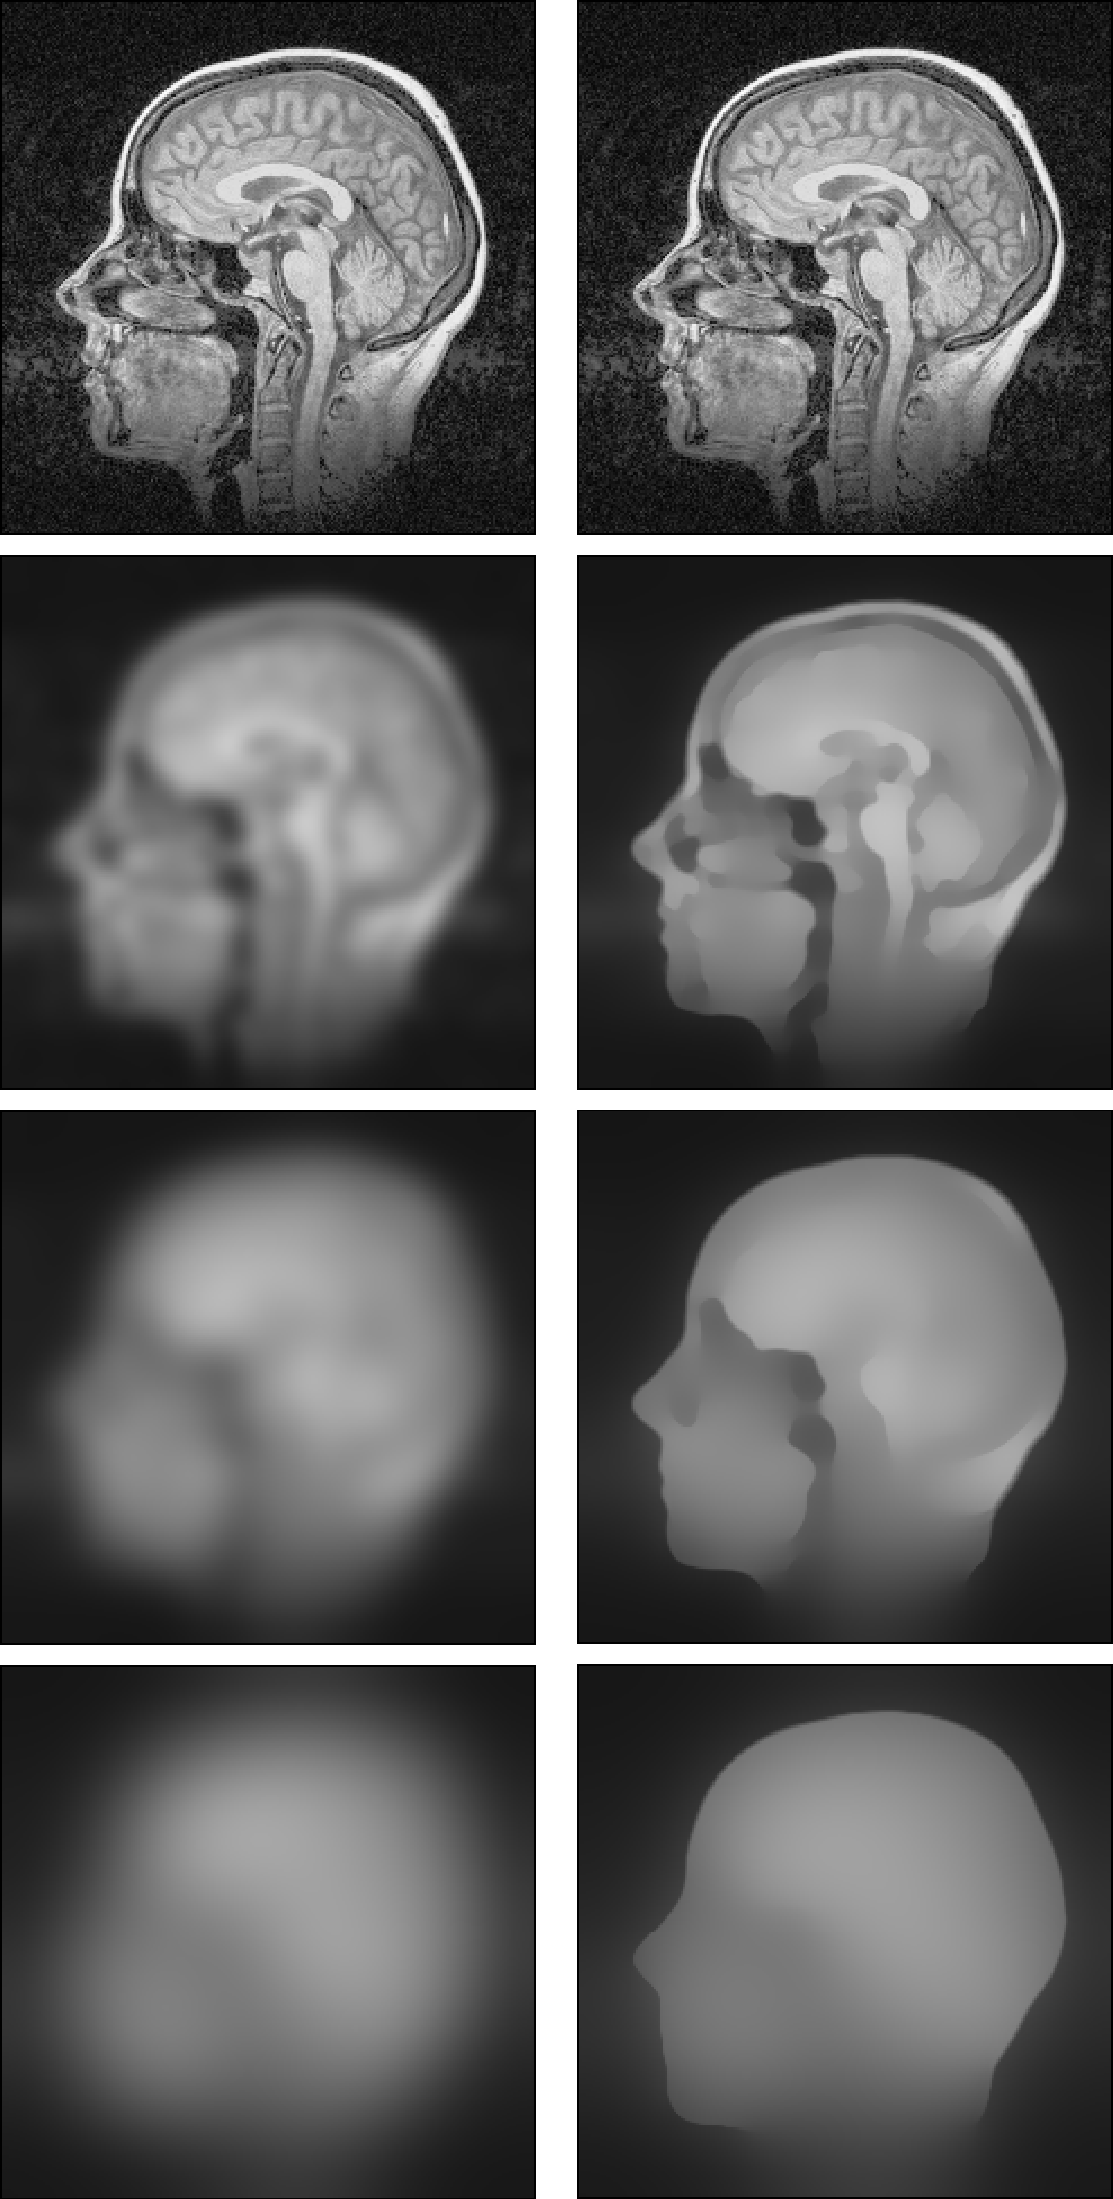
\includegraphics[width=.5\textwidth]{gfx/lin_vs_nonlin_diffusion2.png}
      \caption[Linear vs. nonlinear diffusion]{Image from \citep[p.120,121]{weickert1998}. Linear diffusion on the left,
   anisotropic nonlinear diffusion on the right.}
   \label{fig:lin_vs_nonlin_diffusion}}
\end{figure}

The AKAZE descriptor is obtained from dividing the image region around a
keypoint into a grid and then performing binary tests between all such grid
cells $i,~j$ which test whether $f(i) > f(j)$ for some function $f$ which
encapsulates some information of the cell \citep{yang2012}. To achieve rotation
invariance, this grid is rotated according to the dominant orientation computed
by considering the image derivatives---already computed for the detection---in
the neighbourhood \citep{alcantarilla2012}. The results of these binary tests are
assembled into a binary vector. Its size can be adjusted by making the grid
coarser or finer. For $f$, \citet{alcantarilla2012} consider both intensity
differences and two image derivatives. The three properties are referred to as
\emph{channels} and the descriptor may include one, two or all three of them,
with three yielding best performance.

\section{Practical Problems}
\label{sec:app_challenges}

In the context of a rephotography application as in \citep{bae2010}, five
primary obstacles in viewpoint reconstruction of a historic photograph can be
identified.
\begin{enumerate}
   \item The necessary camera motion has six degrees of freedom---three for
      translation and three for rotation---which are challenging for the user
      to adjust simultaneously, as changing one parameter will often necessitate
      adjustments for the others to improve the registration. Furthermore, the
      number of degrees of freedom makes it difficult to communicate to the
      user how they must move the camera.
   \item Computing relative translation between two cameras from corresponding
      image points is possible only up to an unknown scale (see
      \autoref{sec:eight-point}), meaning it is impossible to
      determine e.g. if an object viewed by the camera is small and close or
      large and further away. This poses the problem of how to determine if the
      user is close to the desired viewpoint and whether or not they have come
      closer or moved further away over iterations. 
   \item Relative pose estimation from corresponding points becomes unstable
      when the motion between the two cameras approaches zero, which is the
      ultimate goal one wishes to achieve, as this is a degenerate configuration
      (see \autoref{subsec:motion_degen}). When na\"ivley comparing the current
      camera image to the reference photograph, the estimate for relative
      rotation and translation would become increasingly unreliable as the
      camera approaches the original viewpoint.
   \item Automated computation of relative camera pose will rely on feature
      detection to find correspondences. However, historical images will often
      be vastly different from the current scene. Not only may the scene itself
      have changed considerably, but also the historical image---having been
      taken by a historical camera---may differ in contrast, sharpness and
      colours. Feature detectors may not be able to reliably find
      correspondences when comparing an old with a new photograph. Neither SIFT
      nor AKAZE will reliably find correspondences with a current photo.
   \item The calibration data---most importantly, focal length and principal
      point---of the historical camera are often unknown. The calibration data
      is needed for relative pose computation (see \autoref{sec:epipolar}).
\end{enumerate}

\citet{bae2010} address all these issues in the following way.
Initially, after loading a historical image, the user is instructed to
take two photographs of the scene with a reasonably wide baseline (about
20\textdegree). One of them, termed \emph{first frame} is supposed to be
taken from some distance from the original viewpoint, the \emph{second
frame} should be the user's best eyeballed approximation of it. The wide
baseline allows for a more reliable 3D-reconstrution of the scene used to
tackle problems 2. and 3. 

SIFT features are computed and matched between the two images.  Given these
correspondences, 3D coordinates of the points can be computed. A selection of
these is reprojected into the second frame after which the user identifies six
or more points in the historical photograph corresponding to these points in the
second frame. This allows estimating extrinsic and intrinsic camera parameters
of the historical camera by running an optimisation algorithm on an initial
estimate for relative rotation and translation between first frame and reference
image as well as sensor skew, focal length and principal point of the historical
camera (problem 5.).  Hence, the reference photograph is not needed anymore
after this initial step, circumventing problem 4.  The principal point's initial
guess is found again with help of the user who identifies three sets of parallel
lines in the historical image \citep[see][chapter 8.8]{h&z2004}.

In this work, this problem is neglected and it is assumed that the original
image can be matched with current photographs, so it should not actually be
historic. This restriction is envisioned to be removed in the future.

The result is that the pose of the reference camera relative to the first
camera $T_{\text ref,first},~R_{\text ref,first}$ is known. During the homing
process, the current camera frame is compared to the first frame (not the
reference frame, avoiding problem 3.), which avoids degeneracy due to the wide
baseline. Thus one obtains $T_{\text current,first},~R_{\text current,first}$.
Given the locations of the reference camera and the current frame's camera, each
relative to the first frame, one can compute the location of the reference
relative to the current frame and thus guide the user in the right direction.

\begin{IEEEeqnarray}{rCllt}
   \sub{X}{ref}      & =  & \sub{R}{ref,first}\sub{X}{first} + \sub{T}{ref,first} & \hspace{1em}\\
   \sub{X}{current}  & =  & \sub{R}{current,first}\sub{X}{first} + \sub{T}{current,first}\\[\baselineskip]
   \sub{X}{first}    & =  & \sub{R^T}{current,first}\left(\sub{X}{current} - \sub{T}{current,first}\right) && (1, $R$ orthogonal)\IEEEnonumber\\
   \sub{X}{ref}      & =  & \sub{R}{ref,first}\sub{R^T}{current,first}\left(\sub{X}{current} - \sub{T}{current,first}\right) \\
                     &    & + \sub{T}{ref,first} & & (2, substitute 1)\IEEEnonumber\\
   \sub{X}{ref}      & =  & \sub{R}{ref,first}\sub{R^T}{current,first}\sub{X}{current} \\
                     &    & - \sub{R}{ref,first}\sub{R^T}{current,first}\sub{T}{current,first} + \sub{T}{ref,first}
\end{IEEEeqnarray}
and thus
\begin{equation}\label{eq:necessary_trans}
   \sub{T}{ref,current} = - \sub{R}{ref,first}\sub{R^T}{current,first}\sub{T}{current,first} + \sub{T}{ref,first}
\end{equation}
and
\begin{equation}\label{eq:necessary_rot}
   \sub{R}{ref,current} = \sub{R}{ref,first}\sub{R^T}{current,first}
\end{equation}

During homing, Bae et. al warp the current camera frame according to the
necessary rotation before being shown to the user, allowing them to focus only
on the translation (problem 1.). This is possible since for rephotography
dealing with structures usually at some distance, the rotation will be small,
otherwise the warped image would be unusable. This simplification is also
disregarded in this work, as achieving the correct rotation with the help of an
overlayed edge image is easy enough, as long as one is directed to the correct
spot. Therefore, only the translation is communicated.

A remaining problem (2.) is that the scale of the necessary translation is
unknown, so that only the direction can be determined. This poses the question
of how to find out whether the user has come closer to the goal or not. It may
be feasible to find the original viewpoint nonetheless, if it could be
determined at least when the user reaches it, but this is not the case without
further information. On top of that, it would make for a better user experience
if also the distance to the goal could be communicated.

A key observation in this regard is that the actual scale of the translation is
irrelevant, it is sufficient that there be a way to make the scale consistent
accross iterations. That is, it is unnecessary to know whether the goal is a
specific distance away, if one can ensure that the translations computed one
after the other can be somehow meaningfully compared. For this, \citet{bae2010}
observe that when triangulating 3D coordinates from corresponding points, their
computed distance from the camera (the first frame) is inversely proportional
to the distance between the cameras. An intuition can be obtained from
\autoref{fig:scale}. To measure the scale of the world, the application uses the
matches between two images and computes 3D coordinates by triangulation. The
average distance of those points to the first frame's camera centre is computed
and compared across iterations to make the scale consistent.

\begin{figure}
   {\centering      
      \begin{subfigure}{\linewidth}
      \begin{tikzpicture}[very thick,node distance=2em]
   \tikzset{>=Latex}
   \def\camAngle{60}
   \def\arrowLength{3em}
   \node[label={180:{$c_1$}}] (c1) at (0,0) {};
   \fill (c1) circle (3pt);
   \node[below left=of c1] {first frame};
   \draw[->] (c1) -- (\camAngle:\arrowLength);
   \node[minimum size=1em,draw,label={90:Object}] (object) at (\camAngle:3cm) {};
   \draw[dashed,name path=line1] (c1) -- (object) node[label={180:{$o_1$}}] {};
   \node[right=3cm of c1,label={0:{$c_2$}}] (c2) {};
   \fill (c2) circle (3pt);
   \draw[->] (c2) -- ($(c2) !3em! (object)$) coordinate (tmp);
   \draw[dashed,name path=line2] (c2) -- (object);
   \node[below right=of c2] {current frame};
   \draw[thin,|-|] ($(c1) + (0,-1em)$) -- ($(c2) + (0,-1em)$) node[below,midway] {$b=1$};

   \draw[thin] (c1) ++(\camAngle:\arrowLength) arc (\camAngle:0:\arrowLength) -- (c1);
   \node at (\camAngle/2:2em) {$\alpha$};

   \pgfmathanglebetweenpoints{\pgfpointanchor{c2}{center}}{\pgfpointanchor{object}{center}}
   \let\reverseAngle\pgfmathresult
   \draw[thin] (tmp) arc (\reverseAngle:180:\arrowLength) -- (c2);
   \pgfmathparse{\reverseAngle+(180-\reverseAngle)/2}
   \node at ($(c2) + (\pgfmathresult:2em)$) {$\beta_1$};

   \coordinate (tmp1) at ($(c1) + (0,1.5cm)$);
   \coordinate (tmp2) at ($(c2) + (0,1.5cm)$);
   \path[name path=second baseline] (tmp1) -- (tmp2);
   \path[name intersections={of=second baseline and line1}] (intersection-1) coordinate (second c1);
   \path[name intersections={of=second baseline and line2}] (intersection-1) coordinate (second c2);
   \fill (second c1) circle (3pt) node[label={180:{$c_1^\prime$}}] {};
   \fill (second c2) circle (3pt) node[label={0:{$c_2^\prime$}}] {};
   \draw[|-|,thin,transform canvas={yshift=-1em}] (second c1) -- (second c2) node[below,midway] {$b^\prime$};

   % \draw[thin,|-|,transform canvas={shift=(90+\camAngle:1em)}] (second c1) -- (object);
\end{tikzpicture}


      \caption{Per the intercept theorem $\frac{|s c_1^\prime|}{|s c_1|} = \frac{b^\prime}{b}$.  
      With increasing baseline, $|s c_1|$ also increases to fulfil the equation.}
      \end{subfigure}

      \begin{subfigure}{\linewidth}
      \begin{tikzpicture}[very thick,node distance=2em]
   \tikzset{>=Latex}
   \def\camAngle{60}
   \def\arrowLength{3em}
   \node[label={180:{$c_1$}}] (c1) at (0,0) {};
   \fill (c1) circle (3pt);
   \node[below left=of c1] {first frame};
   \draw[->] (c1) -- (\camAngle:\arrowLength);
   \node[minimum size=1em,draw] (object) at (\camAngle:3cm) {};
   \draw[dashed,name path=line1] (c1) -- (object) node[label={180:{$o_2$}}] {};
   \node[label={0:{$c_3$}},right=5cm of c1] (c3) {};
   \fill (c3) circle (3pt);
   \draw[->] (c3) -- ($(c3) !3em! (object)$) coordinate (tmp);
   \draw[dashed,name path=line2] (c3) -- (object);
   \node[below right=of c3] {current frame};

   \pgfmathanglebetweenpoints{\pgfpointanchor{c3}{center}}{\pgfpointanchor{object}{center}}
   \let\reverseAngle\pgfmathresult
   \draw[thin] (tmp) arc (\reverseAngle:180:\arrowLength) -- (c3);
   \pgfmathparse{\reverseAngle+(180-\reverseAngle)/2}
   \node at ($(c3) + (\pgfmathresult:2em)$) {$\beta_2$};

   \draw[thin,|-|] ($(c1) + (0,-1em)$) -- ($(c3) + (0,-1em)$) node[below,midway] {$b=1$};

   % \draw[thin,|-|,transform canvas={shift=(90+\camAngle:1em)}] (second c1) -- (object);
\end{tikzpicture}


      \caption{For another baseline, the estimate will still yield a translation
      with unit length.}
      \end{subfigure}

      \begin{subfigure}{\linewidth}
      \begin{tikzpicture}[very thick,node distance=2em]
   \tikzset{>=Latex}
   \def\camAngle{60}
   \def\arrowLength{3em}
   \node[label={180:{$c_1$}}] (c1) at (0,0) {};
   \fill (c1) circle (3pt);
   \node[below left=of c1] {first frame};
   \draw[->] (c1) -- (\camAngle:\arrowLength);
   \node[minimum size=1em,draw] (object) at (\camAngle:3cm) {};
   \draw[dashed,name path=line1] (c1) -- (object) node[label={180:{$s$}}] {};
   \node[label={0:{$c_2$}},right=3cm of c1] (c2) {};
   \fill (c2) circle (3pt);
   \draw[dashed,name path=line2] (c2) -- (object);
   \node[below right=of c2] {current frame};

   \draw[->] (c2) -- ($(c2) !3em! (object)$) coordinate (tmp);


   \draw[thin,|-|] ($(c1) + (0,-1em)$) -- ($(c2) + (0,-1em)$) node[below,midway] {$b=1$};

   % \draw[thin,|-|,transform canvas={shift=(90+\camAngle:1em)}] (second c1) -- (object);

   \begin{scope}[transform canvas={xshift=-2cm}]
      \node[label={180:{$c_3$}},right=5cm of c1] (c3) {};
      \fill (c3) circle (3pt);
      \draw[->] (c3) -- ($(c3) !3em! (object)$) coordinate (tmp);
   \end{scope}
   \coordinate (tmp1) at ($(c3) + (-2cm,0)$);
   \coordinate (tmp2) at ($(tmp) + (-2cm,0)$);
   \path[name path=line3] (tmp1) -- ($(tmp1) !5cm! (tmp2)$);
   \draw[name intersections={of=line1 and line3}]
   node[label={180:{$s_2$}},minimum size=1em,draw,fill=white] (object2) at (intersection-1) {};
   \draw[dashed] (tmp1) -- (object2);
\end{tikzpicture}


      \caption{Equalising the scales in both estimates shows that the distance
      of the object to $c_1$ is smaller if $c_3$ was further away than $c_2$}
      \end{subfigure}

      \caption[Relation between object distance and camera baseline]{The camera
         baseline length is inversely proportional to the distance of the viewed
      object to one of the cameras. Evaluating the distance of viewed objects to
   the first frame's camera yields a measure for how far the two cameras are
apart.}
   \label{fig:scale}}
\end{figure}

Therefore, in each iteration, the scale of the world is computed by
triangulating correspondences between the first and current frames and computing
the average distance to the first frame's camera. The scale is
compared to the scale computed in the initial step for the first and second
frames. Scaling the current translation vector by the ratio of the
two scales makes the length consistent across iterations and decreasing with the
distance to the goal. However, as this estimate relies on the intercept theorem,
it is only valid as long as the user moves on a straight line between the
initial estimate (position of the second frame) and the goal. Empirical
analysis (see evaluation in \autoref{ch:evaluation}) demonstrates that strong
movement along the optical axis will decrease the usefulness of the scale
estimation. However, in reality this should be a minor problem, as the movement
around a scene will be stronger than towards or away from it when
rephotographing.

For a summary, \autoref{fig:procedure} shows how the whole pipeline works.
\begin{figure}[h]
   {\centering      
      \begin{tikzpicture}[
      very thick,
      node distance=1.5cm,
      every node/.append style={font=\small,text width=1.5cm,text centered},
      circle node/.style={inner sep=0,shape=circle,draw},
      boxnode/.style={outer sep=0,inner
         sep=4pt,fill=RoyalBlue,text=white,draw=gray,shape=rectangle,rounded
      corners=5pt,minimum height=1.3cm},
      descision node/.style={diamond,aspect=3,inner sep=5pt,draw,text centered},
   ]

   \makegrayinprint

   \tikzset{>=latex}
   \node[boxnode] (ref) {Reference photo};
   \node[boxnode,right=of ref] (first frame) {First frame};
   \node[boxnode,right=of first frame] (second frame) {Second frame};
   \node[draw] (t first ref) at ($(ref) !.5! (first frame) + (0,-3cm)$) {$T_{\text first,ref}$};

   \node[circle node] (triangulation) at ($(first frame) !.5! (second frame) +
   (0,-3cm)$) {Triangu-lation};

   \coordinate (c) at ($(t first ref.north) + (0,1em)$);

   \node[above] at (c) {\texttt{AKAZE}};
   \draw[->] (ref.south) |- (c) -- (t first ref);
   \draw[->] (first frame.south) |- (c) -- (t first ref);
   \draw (first frame) -- coordinate[midway] (c) (second frame);
   \draw[->] (c) -- (triangulation);
   \draw[->] (triangulation) -- (t first ref);
   \node[above] at (c) {\texttt{AKAZE}};

   \begin{scope}[shift={(0cm,-5cm)}]
      \node[opacity=.5,anchor=north west,inner sep=0] at (0,0) {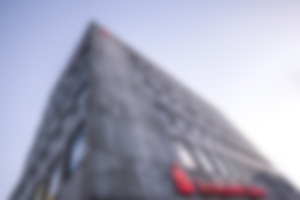
\includegraphics[width=3cm]{gfx/pic.jpg}};
      \draw (0,0) rectangle (3,-2);
      \node (current frame) at (1.5,-0.5) {Current frame};
      \draw[ultra thick,xshift=-1em,->] (1.5,-1.5) -- ++(100:1em);
      \draw[ultra thick,xshift=+1em,->] (1.5,-1.5) -- ++(30:1em);

      \node[circle node,right=of current frame] (triangulation2)
      {Triangu-lation};
      \node[draw,text width={}] (t first current) at ($(current frame) !.5! (triangulation2) +
      (0,-3cm)$) {$T_{\text first,current}$};

      \node[descision node,below=1cm of t first current,inner sep=10pt] (ifequal) {$T_{\text first,current} = T_{\text first,ref}$?};
      \node[boxnode,right=of t first current] (final frame) {Final image};

      \draw[->] (ifequal.west) -- ++(-2cm,0) |- (0,-1) node[midway,left=1em,rotate=90] {No};
      \draw[->] (ifequal.east) -| (final frame.south) node[midway,right=-1em] {Yes};

      \coordinate (c) at ($(t first current.north) + (0,1em)$);
      \draw[->] (c) -- (t first current);
      \draw (triangulation2) |- (c);

      \draw[->] (first frame.north) -- ++(0,1em) -- ++(-5cm,0) -- ++(0,-4cm)
      node[rotate=90,left=1em,midway]
      {\texttt{AKAZE}} |-
      (1.5,1) -| (triangulation2.north);
      \draw[->] (1.5,0) -- ++(0,1);
      \draw (3.5,1) |- (c);
      \draw[->] (t first current) -- (ifequal);

      \draw[|-|] (8.5cm,0) -- ++(0,-6cm) node[right=1em,midway,rotate=90,anchor=center] {Iterate};
   \end{scope}
   \draw[|-|] (8.5cm,1cm) -- ++(0,-4cm) node[right=1em,midway,rotate=90,anchor=center] {Preprocessing};
\end{tikzpicture}

      \caption{Rephotography procedure}
   \label{fig:procedure}}
\end{figure}
